% Flowchart
% Author: Stefan Kottwitz
% https://www.packtpub.com/hardware-and-creative/latex-cookbook
\documentclass[border=20pt]{standalone}
%\usepackage[a0paper,vmargin=3cm]{geometry}
\usepackage[a4paper,vmargin=3cm]{geometry}
%\usepackage{cooltooltips]
%\usepackage{hyperref}
%
%\usepackage{xcolor}
%
%\usepackage{pdfcomment}
% \usepackage{array}
\newcounter{rowno}
\setcounter{rowno}{0}
\newcounter{chptno}
\setcounter{chptno}{0}


\usepackage{tikz}
\usetikzlibrary{matrix,calc,shapes,decorations.pathreplacing,calligraphy}
\tikzset{
  treenode/.style = {shape=rectangle, rounded corners,
	draw, anchor=center,
	text width=12em, align=center,
	top color=white, bottom color=blue!20,
	inner sep=1ex},
%  decision/.style = {treenode, diamond, inner sep=0pt},
  %concept/.style = {treenode, diamond, inner sep=0pt},
  concept/.style = {treenode, bottom color=cyan!30},
  blank/.style = {draw=none, bottom color=white!30, font=\ttfamily\large},
  background/.style      = {treenode, bottom color=red!30},
  %background/.style      = {treenode, bottom color=red!30, font=\ttfamily\small},
  section/.style      = {treenode, bottom color=green!30},
  activity/.style = {treenode, bottom color=yellow!30},
  skill/.style = {treenode, bottom color=blue!30},
  topic/.style = {treenode, bottom color=orange!30},
  part/.style = {treenode, bottom color=magenta!30},
  root/.style     = {treenode, font=\Large, bottom color=yellow!30},
%  env/.style      = {treenode, font=\ttfamily\normalsize},
  finish/.style   = {root, bottom color=green!40},
  dummy/.style    = {circle,draw}
}
\newcommand{\yes}{edge node [above] {yes}}
\newcommand{\no}{edge  node [left]  {no}}
\begin{document}

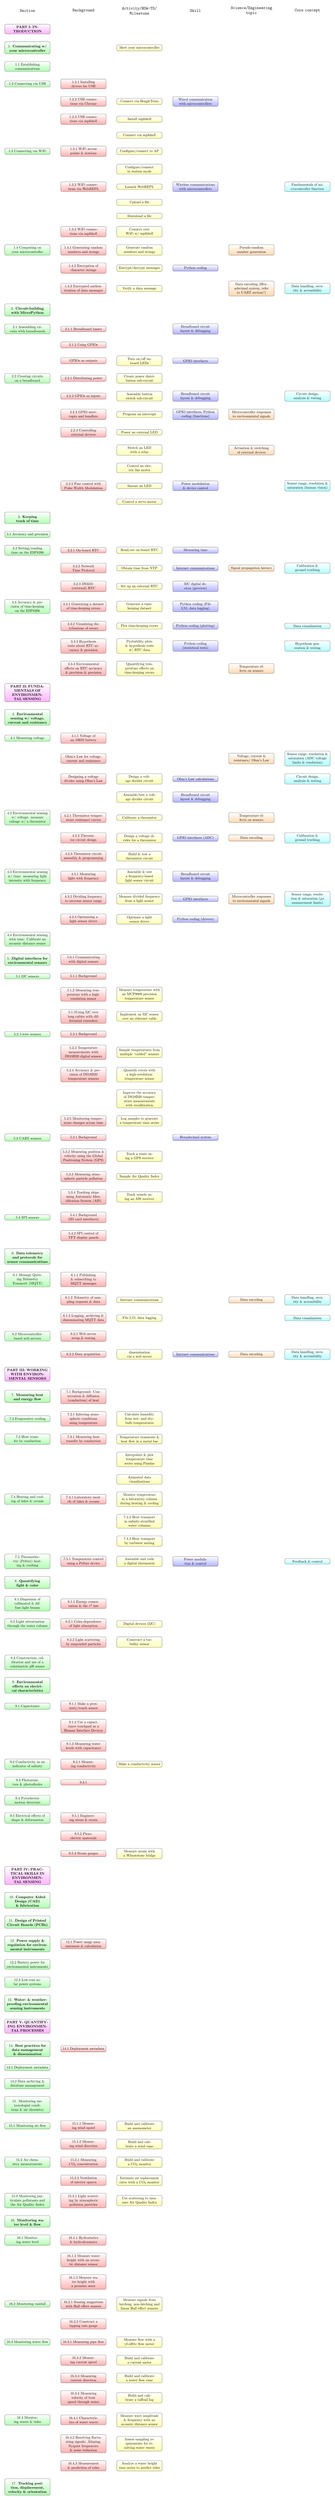
\begin{tikzpicture}[-latex]
  \matrix (chart)
    [
      matrix of nodes,
      %anchor=west,
      column sep      = 3em,
      row sep         = 5ex,
      column 1/.style = {nodes={section}},
      column 2/.style = {nodes={background}},
      column 3/.style = {nodes={activity}},
	    column 4/.style = {nodes={skill}},
      column 5/.style = {nodes={topic}},
	    column 6/.style = {nodes={concept}}
      % ,\stepcounter{rowno}
      % \stepcounter{rowno}\therowno \hspace{1cm}
%      column 7/.style = {nodes={concept}},
%	  column 8/.style = {nodes={section}},
%	  column 9/.style = {nodes={background}}
    ]
    {
      %& &  |[root]| Prosection               \\
      |[blank]|Section     & |[blank]|Background  & |[blank]|Activity/HOW-TO/ Milestone  & |[blank]|Skill &  |[blank]|Science/Engineering topic & |[blank]|Core concept  \\
%
       |[part]| \textbf{PART I: INTRODUCTION}   & &      & &        &      \\

      \stepcounter{chptno}\thechptno. \textbf{Communicating w/ your microcontroller}   & & Meet your microcontroller     & &        &      \\
      % 1. \textbf{Communicating w/ your microcontroller}   & & Meet your microcontroller     & &        &      \\
          \thechptno.1 Establishing communications    &  &    & &        &      \\
          \thechptno.2 Connecting via USB    & \thechptno.2.1 Installing drivers for USB &    & &        &      \\
              & \thechptno.2.2 USB connections via Chrome & Connect via BeagleTerm & Wired communication with microcontrollers &        &      \\
              & \thechptno.2.3 USB connections via mpfshell &   Install mpfshell & &        &      \\
              &  &   Connect via mpfshell & &        &      \\
          \thechptno.3 Connecting via WiFi     & \thechptno.3.1 WiFi access points \& stations &  Configure/connect to AP  &  &        &      \\
                                 &   &  Configure/connect in station mode  & &        &      \\
              & \thechptno.3.2 WiFi connections via WebREPL &  Launch WebREPL  & Wireless communications with microcontrollers &        & Fundamentals of microcontroller function     \\
                                 &   &  Upload a file  & &        &      \\
                                 &   &  Download a file  & &        &      \\
              & \thechptno.3.3 WiFi connections via mpfshell & Connect over WiFi w/ mpfshell  & &        &      \\
      \thechptno.4 Computing on your microcontroller    &  \thechptno.4.1 Generating random numbers and strings &  Generate random numbers and strings  & & Pseudo-random number generation         &      \\
              & \thechptno.4.2 Encryption of character strings &  Encrypt/decrypt messages  & Python coding &        &  \\
              & \thechptno.4.3 Encrypted authentication of data messages &  Verify a data message  & &  Data encoding (Hexadecimal system, refer to UART section?)    &  Data handling, security \& accessibility    \\

      \stepcounter{chptno}\thechptno. \textbf{Circuit-building with MicroPython}   &  &    & &        &      \\
          \thechptno.1 Assembling circuits with breadboards    & \thechptno.1.1 Breadboard basics &    & Breadboard circuit layout \& debugging &        &      \\
              & \thechptno.1.2 Using GPIOs &    & &        &      \\
              &  GPIOs as outputs &  Turn on/off on-board LEDs  & GPIO interfaces &        &      \\
          \thechptno.2 Creating circuits on a  breadboard   & \thechptno.2.1 Distributing power & Create power distribution sub-circuit   & &        &      \\
             & \thechptno.2.2 GPIOs as inputs & Assemble button switch sub-circuit   & Breadboard circuit layout \& debugging &        &  Circuit design, analysis \& testing   \\
             & \thechptno.2.3 GPIO interrupts and handlers & Program an interrupt   & GPIO interfaces, Python coding (functions) &  Microcontroller responses to environmental signals      &      \\
             & \thechptno.2.4 Controlling external devices & Power an external LED   & &        &      \\
             &  & Switch an LED with a relay   &  &  Actuation \& switching of external devices      &      \\
             &  & Control an electric fan motor   &  &        &      \\
             & \thechptno.2.5 Fine control with Pulse Width Modulation & Snooze an LED   & Power modulation \& device control &        & Sensor range, resolution \& saturation (human vision) \\
             &       & Control a servo motor   & &        &  \\

      \stepcounter{chptno}\thechptno. \textbf{Keeping track of time}   &  &    & &        &      \\
          \thechptno.1 Accuracy and precision    &  &    & &        &      \\
          \thechptno.2 Setting/reading time on the ESP8266    & \thechptno.2.1 On-board RTC & Read/set on-board RTC   & Measuring time &        &      \\
              & \thechptno.2.2 Network Time Protocol  & Obtain time from NTP   & Internet communications &  Signal propagation latency  & Calibration \& ground truthing     \\
              & \thechptno.2.3 DS3231 (external) RTC & Set up an external RTC   & I2C digital devices (preview) &       &      \\
      \thechptno.3 Accuracy \& precision of time-keeping on the ESP8266    & \thechptno.3.1 Generating a dataset of time-keeping errors & Generate a time-keeping dataset   & Python coding (File I/O, data logging) &          \\
              & \thechptno.3.2 Visualizing distributions of errors  & Plot time-keeping errors   & Python coding (plotting) &        & Data visualization     \\
              & \thechptno.3.3 Hypothesis tests about RTC accuracy \& precision  & Probability plots \& hypothesis tests w/ RTC data   & Python coding (statistical tests) &   & Hypothesis generation \& testing \\
              & \thechptno.3.4 Environmental effects on RTC accuracy \& precision \& precision  & Quantifying temperature effects on time-keeping errors   & & Temperature effects on sensors  &      \\
%
%
       |[part]| \textbf{PART II: FUNDAMENTALS OF ENVIRONMENTAL SENSING}   & &      & &        &      \\

      \stepcounter{chptno}\thechptno. \textbf{Environmental sensing w/ voltage, current and resistance}   &  &    & &        &      \\
          \thechptno.1 Measuring voltage    & \thechptno.1.1 Voltage of an 18650 battery &    & &        &      \\
              & Ohm's Law for voltage, current and resistance &    & & Voltage, current \& resistance/ Ohm's Law   &   Sensor range, resolution \& saturation (ADC voltage limits \& resolution)   \\
              & Designing a voltage divider using Ohm's Law & Design a voltage divider circuit   & Ohm's Law calculations  &        & Circuit design, analysis \& testing     \\
              &  & Assemble/test a voltage divider circuit   & Breadboard circuit layout \& debugging &        &   \\
          \thechptno.2 Environmental sensing w/ voltage: measure voltage w/ a thermistor    & \thechptno.2.1 Thermistor temperature resistance curves & Calibrate a thermistor   & &   Temperature effects on sensors     &      \\
              & \thechptno.2.2 Thermistor circuit design & Design a voltage divider for a thermistor   & GPIO interfaces (ADC) &  Data encoding  &  Calibration \& ground truthing    \\
              & \thechptno.2.3 Thermistor circuit assembly \& programming & Build \& test a thermistor circuit   & &        &      \\
          \thechptno.3 Environmental sensing w/ time: measuring light intensity with frequency    & \thechptno.3.1 Measuring light with frequency & Assemble \& test a frequency-based light sensor circuit   & Breadboard circuit layout \& debugging &        &      \\
              & \thechptno.3.2 Dividing frequency to increase sensor range & Measure divided frequency from a light sensor   & GPIO interfaces & Microcontroller responses to environmental signals       &      Sensor range, resolution \& saturation ($\mu s$ measurement limits)\\
              & \thechptno.3.3 Optimizing a light sensor driver & Optimize a light sensor driver   & Python coding (drivers) &        &      \\
          \thechptno.4 Environmental sensing with time: Calibrate an acoustic distance sensor   &  &      \\

      \stepcounter{chptno}\thechptno. \textbf{Digital interfaces for environmental sensors}   & \thechptno.0.1 Communicating with digital sensors &    & &        &      \\
          \thechptno.1 I2C sensors   & \thechptno.1.1 Background &      \\
             & \thechptno.1.2 Measuring temperature with a high-resolution sensor   & Measure temperature with an MCP9808 precision temperature sensor &        &    \\
             & \thechptno.1.\thechptno Using I2C over long cables with differential extenders   & Implement an I2C sensor over an ethernet cable &        &    \\
          \thechptno.2 1-wire sensors   &  \thechptno.2.1 Background &      \\
             & \thechptno.2.2 Temperature measurements with DS18B20 digital sensors &  Sample temperatures from multiple ``cabled'' sensors   &  &        &    \\
             & \thechptno.2.4 Accuracy \& precision of DS18B20 temperature sensors & Quantify errors with a high-resolution temperature sensor   &   &        &    \\
             &  & Improve the accuracy of DS18B20 temperature measurements with recalibration   &   &        &    \\
             & \thechptno.2.5 Monitoring temperature changes across time & Log samples to generate a temperature time series   &   &        &    \\

          \thechptno.3 UART sensors   &  \thechptno.3.1 Background &   & Hexadecimal system   \\
             & \thechptno.3.2 Measuring position \& velocity using the Global Positioning System (GPS) &  Track a route using a GPS receiver  &  &        &    \\
             & \thechptno.3.3 Measuring atmospheric particle pollution &  Sample Air Quality Index   &  &        &    \\
             & \thechptno.3.4 Tracking ships using Automatic Identification System (AIS) &  Track vessels using an AIS receiver  &  &        &    \\
          \thechptno.4 SPI sensors   &  \thechptno.4.1 Background (SD card interfaces)&      \\
             & \thechptno.4.2 SPI control of TFT display panels &    &  &        &    \\

      \stepcounter{chptno}\thechptno. \textbf{Data telemetry and protocols for sensor communications}   &  &    & &        &      \\
          \thechptno.1 Message Queuing Telemetry Transport (MQTT)    & \thechptno.1.1 Publishing \& subscribing to MQTT messages &    & &        &      \\
             & \thechptno.1.2 Telemetry of sampling requests \& data &  Internet communications   &  &  Data encoding      &   Data handling, security \& accessibility   \\
             & \thechptno.1.3 Logging, archiving \& disseminating MQTT data  & File I/O, data logging    & &        &  Data visualization    \\
          \thechptno.2 Microcontroller-based web servers   & \thechptno.2.1 Web server setup \& testing &    & &        &      \\
             & \thechptno.2.2 Data acquisition & dissemination via a web server &  Internet communications   & Data encoding &   Data handling, security \& accessibility   \\
%
%
       |[part]| \textbf{PART III: WORKING WITH ENVIRONMENTAL SENSORS}   & &      & &        &      \\

      \stepcounter{chptno}\thechptno. \textbf{Measuring heat and energy flow}   & \thechptno.1 Background: Conservation \& diffusion (conduction) of heat  &    & &        &      \\
          \thechptno.2 Evaporative cooling & \thechptno.2.1 Inferring atmospheric conditions using temperature & Calculate humidity from wet- and dry-bulb temperatures   &  &        &    \\
          \thechptno.3 Heat transfer by conduction & \thechptno.3.1 Measuring heat transfer by conduction   &  Temperature transients \& heat flow in a metal bar &        &    \\
                 &  & Interpolate \& plot temperature time series using Pandas  &   &        &    \\
                 &  & Animated data visualizations  &   &        &    \\
          \thechptno.4 Heating and cooling of lakes \& oceans & \thechptno.4.1 Laboratory models of lakes \& oceans & Monitor temperature in a laboratory column during heating \& cooling   &  &        &    \\
                 & & \thechptno.4.2 Heat transport in salinity-stratified water columns   &  &        &    \\
                 & & \thechptno.4.3 Heat transport by turbuent mixing   &  &        &    \\
          \thechptno.5 Thermoelectric (Peltier) heating \& cooliing & \thechptno.5.1 Temperature control using a Peltier device & Assemble and code a digital thermostat  & Power modulation \& control & & Feedback \& control   \\

      \stepcounter{chptno}\thechptno.  \textbf{Quantifying light \& color}   &  &    & &        &      \\
          \thechptno.1 Dispersion of collimated \& diffuse light beams  & \thechptno.1.1 Energy conservation \& the $r^2$ law &    &    &    \\
          \thechptno.2 Light attentuation through the water column & \thechptno.2.1 Color-dependence of light absorption  & Digital devices (I2C) &        &    \\
                 &  \thechptno.2.2  Light scattering by suspended particles & Construct a turbidity sensor   &  &        &    \\
                % &  \thechptno.2.3 Light scattering by atmospheric pollution particles & Use scattering to measure Air Quality Index   &  &        &    \\
          \thechptno.3 Construction, calibration and use of a colorimetric pH sensor   &       \\

      \stepcounter{chptno}\thechptno.  \textbf{Environmental effects on electrical characteristics}   &  &    & &        &      \\
          \thechptno.1 Capacitance  & \thechptno.1.1  Make a proximity/touch sensor &    &    &    \\
                 & \thechptno.1.2  Use a capacitance touchpad as a Human Interface Devices  &    &    &    \\
                 & \thechptno.1.3  Measuring water levels with capacitance  &    &    &    \\
          \thechptno.2 Conductivity as an indicator of salinity  & \thechptno.2.1  Measuring conductivity & Make a conductivity sensor     &    &    \\
          \thechptno.3 Photoresistors \& photodiodes  & \thechptno.3.1  & & & & \\
          \thechptno.4 Pyroelectric motion detectors  & &    &    &    \\
          \thechptno.5 Electrical effects of shape \& deformation & \thechptno.5.1 Engineering stress \& strain & & & & \\
                 & \thechptno.5.2 Piezo-electric materials & & & & \\
                 & \thechptno.5.3 Strain gauges & Measure strain with a Wheatstone bridge & & & \\
%
%
       |[part]| \textbf{PART IV: PRACTICAL SKILLS IN ENVIRONMENTAL SENSING}   & &      & &        &      \\

      \stepcounter{chptno}\thechptno.  \textbf{Computer Aided Design (CAD) \& fabrication} & & & & & \\

      \stepcounter{chptno}\thechptno.  \textbf{Design of Printed Circuit Boards (PCBs)} & & & & & \\

      \stepcounter{chptno}\thechptno.  \textbf{Power supply \& regulation for environmental instruments} & \thechptno.1 Power usage measurement \& calculation & & & & \\
          \thechptno.2 Battery power for environmental instruments & & & & & \\
          \thechptno.3 Low-cost solar power systems & & & & & \\

      \stepcounter{chptno}\thechptno.  \textbf{Water- \& weather-proofing environmental sensing instruments} & & & & & \\
%
%
       |[part]| \textbf{PART V: QUANTIFYING ENVIRONMENTAL PROCESSES}   & &      & &        &      \\

      \stepcounter{chptno}\thechptno. \textbf{Best practices for data management \& dissemination}   & \thechptno.1 Deployment metadata  &    & &        &      \\
          \thechptno.1 Deployment metadata  &    & &        &      \\
          \thechptno.2 Data archiving \& database management & & & & & \\

      \stepcounter{chptno}\thechptno. Monitoring meteorologial conditions \& air chemistry & & & & & \\
          \thechptno.1 Monitoring air flow & \thechptno.1.1 Measuring wind speed   & Build and calibrate an anemometer &      \\
                 & \thechptno.1.2 Measuring wind direction   & Build and calibrate a wind vane &      \\
          \thechptno.2 Air chemistry measurements & \thechptno.2.1 Measuring $CO_2$ concentration   & Build and calibrate a $CO_2$ monitor &      \\
                 & \thechptno.2.2 Ventilation of interior spaces   & Estimate air replacement rates with a $CO_2$ monitor &      \\
          \thechptno.3 Monitoring particulate pollutants and the Air Quality Index  &  \thechptno.3.1 Light scattering by atmospheric pollution particles & Use scattering to measure Air Quality Index   &  &        &    \\

      \stepcounter{chptno}\thechptno. \textbf{Monitoring water level \& flow}   &  &    & &        &      \\
          \thechptno.1 Monitoring water level  & \thechptno.1.1 Hydrostatics \& hydrodynamics & & & & \\
                 & \thechptno.1.2 Measure water height with an acoustic distance sensor & & & & \\
                 & \thechptno.1.3 Measure water height with a pressure sesor & & & & \\
          \thechptno.2 Monitoring rainfall   & \thechptno.2.1 Sensing magnetism with Hall effect sensors & Measure signals from latching, non-latching and linear Hall effect sensors   & &        &      \\
                 & \thechptno.2.2 Construct a tipping rain gauge & & & & \\
          \thechptno.3 Monitoring water flow  & \thechptno.3.1 Measuring pipe flow   & Measure flow with a yf-s201c flow meter &      \\
                 & \thechptno.3.2 Measuring current speed   & Build and calibrate a current meter &      \\
                 & \thechptno.3.3 Measuring current direction   & Build and calibrate a water flow vane &      \\
                 & \thechptno.3.4 Measuring velocity of boat speed through water  & Build and calibrate a taffrail log &      \\
          \thechptno.4 Monitoring waves \& tides   & \thechptno.4.1 Characteristics of water waves & Measure wave amplitude \& frequency with an acoustic distance sensor  & &        &      \\
                 & \thechptno.4.2 Resolving fluctuating signals: Aliasing, Nyquist frequencies \& noise reduction & Assess sampling requirements for resolving water waves & & & \\
                 & \thechptno.4.3 Measurement \& prediction of tides & Analyze a water height time series to predict tides & & & \\



      \stepcounter{chptno}\thechptno.  \textbf{Tracking position, displacement, velocity \& orientation} & & & & & \\
};
% % Simple brace
% \draw [-,decorate,
%     decoration = {brace,mirror}] (chart-1-4)[left=] --  (chart-5-4)[midway,left];
%     % decoration = {brace,mirror}] (chart-1-4) --  (chart-5-4)[midway,left];
%
% % Calligraphic brace
% \draw [-,ultra thick,,decorate,
%     decoration = {calligraphic brace,mirror}] (0.2,1) --  (1.2,1);
% %      aligned at relation sign?  & align, flalign \\
% %      aligned at several places? & alignat        \\
% %      first left, centered,
% %        last right?              & multline       \\
% %      & & |[concept]| replicate \\
% %      & & |[treenode]| Add a \texttt{*} & |[finish]| Hypoth. Test \\
% %      & &  \\
% %    };
%   \draw[-]
% %    (chart-1-3) edge node [above] {data} (chart-2-1);
%     (chart-1-3) edge (chart-2-1)
%     (chart-1-3) edge (chart-2-3);
\end{tikzpicture}
\end{document}

  \draw
%    (chart-1-3) edge node [above] {data} (chart-2-1);
    (chart-1-3) edge (chart-2-1)
    (chart-1-3) edge (chart-2-3)
    (chart-1-3) edge (chart-2-5)
    (chart-2-1) edge (chart-3-1)
    (chart-2-3) edge (chart-3-3)
    (chart-2-5) edge (chart-3-5)
    (chart-4-1) edge node [above] {\hspace{1in} uncompress log section} (chart-5-2)
    (chart-4-3) edge node [above] {\hspace{2in} construct full frame from ROIs} (chart-5-4)
    (chart-3-1) edge (chart-4-1)
    (chart-3-3) edge (chart-4-3)
    (chart-3-5) edge (chart-4-5)
    (chart-5-2) edge (chart-6-1)
    (chart-5-4) edge (chart-6-3)
    (chart-6-1) edge node [above] {\hspace{1.5in} parse aqdp data from log section} (chart-7-2)
    (chart-6-3) edge (chart-7-4)
    (chart-7-2) edge node [below] {\hspace{1.25in} record data start/stop times} (chart-8-1)
    (chart-7-4) edge (chart-8-3)
    (chart-9-2) edge node [below] {\hspace{2in} record prosection start/stop times} (chart-10-1)
    (chart-8-1) edge node [above] {\hspace{2in} detect min/max depth in aqdp data} (chart-9-2)
    (chart-4-5) edge node [right] {\hspace{0in} detect min/max depth in CTD data} (chart-9-4)
    (chart-10-1) edge node [above] {\hspace{1.25in} extract data timestamp} (chart-11-2)
    (chart-9-4) edge node [above] {\hspace{2.25in} create section with timestamp in name} (chart-10-5)
    (chart-10-5) edge (chart-11-4)
    (chart-11-2) edge node [above] {\hspace{2.5in} find photo dir matching timestamp} (chart-12-3)
    (chart-11-4) edge node [above] {\hspace{2.25in} create list of matched aqdp/CTD data} (chart-12-5)


    ;
%    (chart-4-2) edge (chart-4-1);
%    (chart-1-2) edge (chart-2-7)8
%    \foreach \x/\y in {2/3, 3/4, 4/5, 5/6} {
%      (chart-\x-1) \no (chart-\y-1) }
%    %\foreach \x in {2,...,6} {
%    \foreach \x in {3,...,6} {
%    	   (chart-\x-1) \yes (chart-\x-2) }
%   (chart-7-3) \no  (chart-8-3)
%   (chart-8-3) edge (chart-8-4);
 \draw
   (chart-8-3) -- +(0,-5) |- (chart-11-2)
   (chart-10-1) -- +(13,0) |- (chart-11-4);
%     node[near start,sloped,above] {no, reconsider};
%  \foreach \x in {3,...,6} {
%   \draw (chart-\x-2) -| (chart-7-3);}
% \draw   (chart-7-3)  -| (chart-8-4)
%   node[near start,above] {yes};
\end{tikzpicture}
\end{document}
